% =============================================================
%  Chapter -- Semiconductor and Cooling
%  The chapter heading and introduction; one file per subsection:
%    semiconductor.tex  module data, on-state model fitted to the
%                       datasheet (Table onstate), ratings
%    die-losses.tex     losses of the four dies of a submodule
%    cooling.tex        cold plate and water path
%    junction.tex       Foster model, periodic steady state
%    example.tex        worked example (Tables modules, dies, flow;
%                       Figure junction waveforms)
%  Figures and tables: fig/, generated by fig/thermal_example.py from
%  tools/example_data.py.
%  Sources: [1] hvdc_lf, src/hvdc_lf/components/semiconductor,
%  components/converter/calc.py (die_losses, periodic_rise, thermal);
%  [2] CM1000HG-130XA datasheet; [3] Dittus and Boelter.
% =============================================================
\section{Semiconductor and Cooling}
\label{sec:thermal}

The semiconductor is the IGBT module with its anti-parallel diode at one switch position of a submodule. Its data
--- ratings, on-state model, switching energies and thermal model --- are a component of their own, taken from the
datasheet at one junction temperature. The converter links to it and adds the number of modules in parallel, the
switching frequency and the cold plate. With these data the converter calculates the losses of
Section~\ref{sec:converter-losses} and the junction temperatures of the dies in the periodic steady state of one
period, without time integration.

\subsection{Semiconductor Data}
\label{sec:semiconductor}

The example module is the Mitsubishi Electric CM1000HG-130XA, 6.5\,kV, 1000\,A, with the data at
$T_j = 125\,^{\circ}$C~[2]. The on-state voltage of IGBT and diode is modelled per module as
\begin{equation}
  v_{CE} = v_{0\_igbt} + r_{igbt} \cdot i_C , \qquad v_{EC} = v_{0\_diode} + r_{diode} \cdot i_E ,
\end{equation}
fitted through the datasheet values at 1000\,A ($V_{CE\_sat} = 3.25$\,V, $V_{EC} = 2.80$\,V, typical, $T_j = 125\,^{\circ}$C)
and the typical output characteristics at 500\,A. This gives $v_{0\_igbt} = 1.45$\,V, $r_{igbt} = 1.80$\,m$\Omega$,
$v_{0\_diode} = 1.60$\,V and $r_{diode} = 1.20$\,m$\Omega$. Table~\ref{tab:onstate} compares the model with the
datasheet: the deviation is at most 0.1\,V from 250\,A to 1000\,A, which covers the module currents of the converter
(up to 0.69\,kA per module in the example), and reaches 0.5\,V at 2000\,A. The points other than 1000\,A are read
from the characteristics with an accuracy of about $\pm 0.1$\,V.

\begin{table}[!ht]
  \centering
  \small
  \begin{tabular}{@{}l r r r r@{}}
    \toprule
    \textbf{Device} & \multicolumn{1}{c}{\textbf{$i$ [kA]}} & \multicolumn{1}{c}{\textbf{Datasheet [V]}}
      & \multicolumn{1}{c}{\textbf{Model [V]}} & \multicolumn{1}{c}{\textbf{Deviation [V]}} \\
    \midrule
    \tablerows{thermal/fig/onstate_table}
    \bottomrule
  \end{tabular}
  \caption{On-state model of the CM1000HG-130XA against the datasheet, $T_j = 125\,^{\circ}$C~[2]}
  \label{tab:onstate}
\end{table}

The switching energies per pulse are those of the datasheet at $V_{CC} = 3600$\,V, $I_C = 1000$\,A,
$R_{G\_on} = 4.3\,\Omega$, $R_{G\_off} = 39\,\Omega$, $L_s = 150$\,nH and $T_j = 125\,^{\circ}$C, as defined in
IEC 60747: $E_{on} = 11.0$\,J, $E_{off} = 7.5$\,J, $E_{rec} = 5.1$\,J~[2]. The converter scales them linearly with
voltage and current (Section~\ref{sec:converter-losses}). The datasheet curves of the energies against current are
not linear; below 1000\,A the linear scaling gives lower energies than the curves.

The thermal data are $R_{th\_jc} = 10.0$\,K/kW (IGBT) and 16.0\,K/kW (diode), maximum values, the contact resistance
case to heat sink $R_{th\_cs} = 5.0$\,K/kW per module (typical, grease $\lambda = 1$\,W/(m$\cdot$K), 80\,$\mu$m), the
highest operating junction temperature $T_{jop} = 150\,^{\circ}$C, and the Foster model of the transient thermal
impedance junction to case, the same for IGBT and diode:
\begin{equation}
  Z_{th\_jc}(t) = R_{th\_jc} \cdot \sum_{i=1}^{4} r_i \cdot \left( 1 - \mathrm{e}^{-t/\tau_i} \right) ,
\end{equation}
with $r_i = 0.0096$, 0.1893, 0.4044, 0.3967 and $\tau_i = 0.1$\,ms, 5.8\,ms, 60.2\,ms, 351.2\,ms~[2].

With the ratings given, the converter warns when the highest submodule capacitor voltage reaches the blocking
voltage $V_{CES}$ and when the peak current per module $I_{arm\_peak} / n_{par}$ exceeds the rated collector current
$I_C$. With one module per switch position the example exceeds $I_C$ (1.38\,kA); with two it does not.

\subsection{Losses of the Dies}
\label{sec:die-losses}

The junction temperatures need the losses of each of the four dies T1, D1, T2, D2 of a submodule separately. The
losses of Section~\ref{sec:converter-losses} are assigned to the dies of the average submodule of an arm, which is
inserted for the share $n_{ins}(t) / N$ of the time. With the current of one module $i_m = |i_{arm}| / n_{par}$,
\begin{equation}
  p_{cond\_igbt} = v_{0\_igbt} \cdot i_m + r_{igbt} \cdot i_m^2 , \qquad
  p_{cond\_diode} = v_{0\_diode} \cdot i_m + r_{diode} \cdot i_m^2 ,
\end{equation}
and the switching powers of one module
\begin{equation}
  p_{sw\_igbt} = f_{sw} \cdot (E_{on} + E_{off}) \cdot \frac{u_{sm}}{U_{sw\_ref}} \cdot \frac{i_m}{I_{sw\_ref}} , \qquad
  p_{sw\_diode} = f_{sw} \cdot E_{rec} \cdot \frac{u_{sm}}{U_{sw\_ref}} \cdot \frac{i_m}{I_{sw\_ref}} ,
\end{equation}
the dies of one module carry, for each sample of the period,
\begin{center}
  \begin{tabular}{@{}l l l@{}}
    \toprule
    & \textbf{Charging current ($-i_{arm} > 0$)} & \textbf{Discharging current} \\
    \midrule
    T1 & 0 & $\frac{n_{ins}}{N} \cdot p_{cond\_igbt} + p_{sw\_igbt}$ \\
    D1 & $\frac{n_{ins}}{N} \cdot p_{cond\_diode} + p_{sw\_diode}$ & 0 \\
    T2 & $\left( 1 - \frac{n_{ins}}{N} \right) \cdot p_{cond\_igbt} + p_{sw\_igbt}$ & 0 \\
    D2 & 0 & $\left( 1 - \frac{n_{ins}}{N} \right) \cdot p_{cond\_diode} + p_{sw\_diode}$ \\
    \bottomrule
  \end{tabular}
\end{center}
With charging current the IGBT T2 switches and the diode D1 recovers; with discharging current T1 switches and D2
recovers. The sum over the dies of all $6 \cdot N \cdot n_{par}$ modules equals the conduction and switching losses
of the converter. The upper and lower arms of a phase are calculated both; the temperatures are reported for the
hotter one.

\subsection{Cold Plate and Water Path}
\label{sec:cooling}

Each submodule sits on one liquid-cooled cold plate. The heat capacity of the plate and the water keeps the heat sink
temperature constant over one period, so the cooling path is calculated with the mean losses of the period. The
$n_{par}$ modules in parallel at a switch position have parallel water paths with the flow $Q_w / n_{par}$ each,
$Q_w$ the flow per cold plate. Along one path the water passes the module of one switch position and then the module
of the other (T1/D1 first in the example), so the second module sees water warmed by the first.

The thermal resistance heat sink to water under one module is one value of the converter design, $R_{th\_hw\_ref}$
at the reference flow $Q_{ref}$, with the flow dependence of the heat transfer coefficient in turbulent flow~[3]:
\begin{equation}
  R_{th\_hw}(Q_w) = R_{th\_hw\_ref} \cdot \left( \frac{Q_{ref}}{Q_w} \right)^{0.8} .
\end{equation}
The example uses $R_{th\_hw\_ref} = 6$\,K/kW at $Q_{ref} = 10$\,l/min, a value to be replaced by the data of the
cold plate. For module $j$ along the path with the mean losses $P_j$ (IGBT and diode),
\begin{align}
  \Delta T_{w\_j} &= \frac{P_j}{\rho \cdot c_p \cdot Q_w / n_{par}} , &
  T_{w\_j} &= T_{w\_in} + \sum_{i<j} \Delta T_{w\_i} + \frac{\Delta T_{w\_j}}{2} , \\
  T_{hs\_j} &= T_{w\_j} + P_j \cdot R_{th\_hw}(Q_w) , &
  T_{case\_j} &= T_{hs\_j} + P_j \cdot R_{th\_cs} ,
\end{align}
with $\rho \cdot c_p = 4.13$\,kJ/(l$\cdot$K) for water at about 50\,$^{\circ}$C ($988\,\mathrm{kg/m^3} \cdot
4.18\,\mathrm{kJ/(kg \cdot K)}$) and $T_{w\_j}$ the mean water temperature along the module. The water inlet
temperature $T_{w\_in}$ (default 50\,$^{\circ}$C) and the flow per cold plate $Q_w$ (default $Q_{ref}$) are part of the
operating point. The water outlet temperature follows from the losses of the cold plate,
$T_{w\_out} - T_{w\_in} = P_{plate} / (\rho \cdot c_p \cdot Q_w)$.

\subsection{Junction Temperature}
\label{sec:junction}

The junction temperature of a die is the case temperature plus the rise across the Foster network of
Section~\ref{sec:semiconductor}, driven by the die losses $p(t)$ of Section~\ref{sec:die-losses}. The losses are
periodic, so the temperatures are as well, and the network is linear. Each Foster element $R_i = r_i \cdot R_{th\_jc}$,
$\tau_i$ is solved exactly for losses that are constant within each of the $M$ samples of length
$\Delta t = 1 / (f \cdot M)$:
\begin{equation}
  \vartheta_i(n+1) = a_i \cdot \vartheta_i(n) + (1 - a_i) \cdot R_i \cdot p(n) , \qquad
  a_i = \mathrm{e}^{-\Delta t / \tau_i} .
\end{equation}
The periodic steady state requires $\vartheta_i(M) = \vartheta_i(0)$, which gives the start value directly:
\begin{equation}
  \vartheta_i(0) = \frac{\sum_{n=0}^{M-1} a_i^{M-1-n} \cdot (1 - a_i) \cdot R_i \cdot p(n)}{1 - a_i^M} .
\end{equation}
One pass over the period from this start value gives the temperature rise; no transient has to settle. The
junction temperature is
\begin{equation}
  T_j(n) = T_{case} + \sum_{i=1}^{4} \vartheta_i(n) .
\end{equation}
Its mean over the period is $T_{case} + R_{th\_jc} \cdot \overline{p}$. The two short time constants (0.1\,ms and
5.8\,ms) set the ripple over the 16.7\,ms period at 60\,Hz; the long ones (60\,ms, 351\,ms) mainly add to the mean.
A junction temperature above $T_{jop}$ is a warning.

The model holds the loss data at the junction temperature of the semiconductor data (125\,$^{\circ}$C); the
dependence of the losses on the calculated junction temperature is not iterated. $R_{th\_jc}$ is a maximum value of
the datasheet, so the junction temperatures are upper values for the given losses.

\subsection{Worked Example}
\label{sec:thermal-example}

At the converter operating point of Section~\ref{sec:converter-example}, with $T_{w\_in} = 50\,^{\circ}$C and
$Q_w = 10$\,l/min per cold plate, the cold plate carries $\thPplate$\,kW and the water leaves it at
$\thTout\,^{\circ}$C. Table~\ref{tab:thermal-modules} gives the temperatures along one water path and
Table~\ref{tab:thermal-dies} the losses and junction temperatures of the dies, for the \thArm{} arm. The hottest die
is \thHot{} at $\thTjmax\,^{\circ}$C. Figure~\ref{fig:junction} shows the losses and junction temperatures of the
four dies over one period.

\begin{table}[!ht]
  \centering
  \small
  \begin{tabular}{@{}l r r r r r@{}}
    \toprule
    \textbf{Module} & \multicolumn{1}{c}{\textbf{Order}} & \multicolumn{1}{c}{\textbf{$P_j$ [kW]}}
      & \multicolumn{1}{c}{\textbf{$T_w$ [$^{\circ}$C]}} & \multicolumn{1}{c}{\textbf{$T_{hs}$ [$^{\circ}$C]}}
      & \multicolumn{1}{c}{\textbf{$T_{case}$ [$^{\circ}$C]}} \\
    \midrule
    \tablerows{thermal/fig/modules_table}
    \bottomrule
  \end{tabular}
  \caption{Temperatures along one water path of the cold plate, example at $T_{w\_in} = 50\,^{\circ}$C,
           $Q_w = 10$\,l/min}
  \label{tab:thermal-modules}
\end{table}

\begin{table}[!ht]
  \centering
  \small
  \begin{tabular}{@{}l r r r r r@{}}
    \toprule
    \textbf{Die} & \multicolumn{1}{c}{\textbf{$\overline{p}$ [kW]}} & \multicolumn{1}{c}{\textbf{$p_{max}$ [kW]}}
      & \multicolumn{1}{c}{\textbf{$\overline{T_j}$ [$^{\circ}$C]}} & \multicolumn{1}{c}{\textbf{$T_{j\_max}$ [$^{\circ}$C]}}
      & \multicolumn{1}{c}{\textbf{$\Delta T_{j\_pp}$ [K]}} \\
    \midrule
    \tablerows{thermal/fig/dies_table}
    \bottomrule
  \end{tabular}
  \caption{Losses and junction temperatures of the dies of one module per switch position, example as in
           Table~\ref{tab:thermal-modules}}
  \label{tab:thermal-dies}
\end{table}

\begin{figure}[!ht]
  \centering
  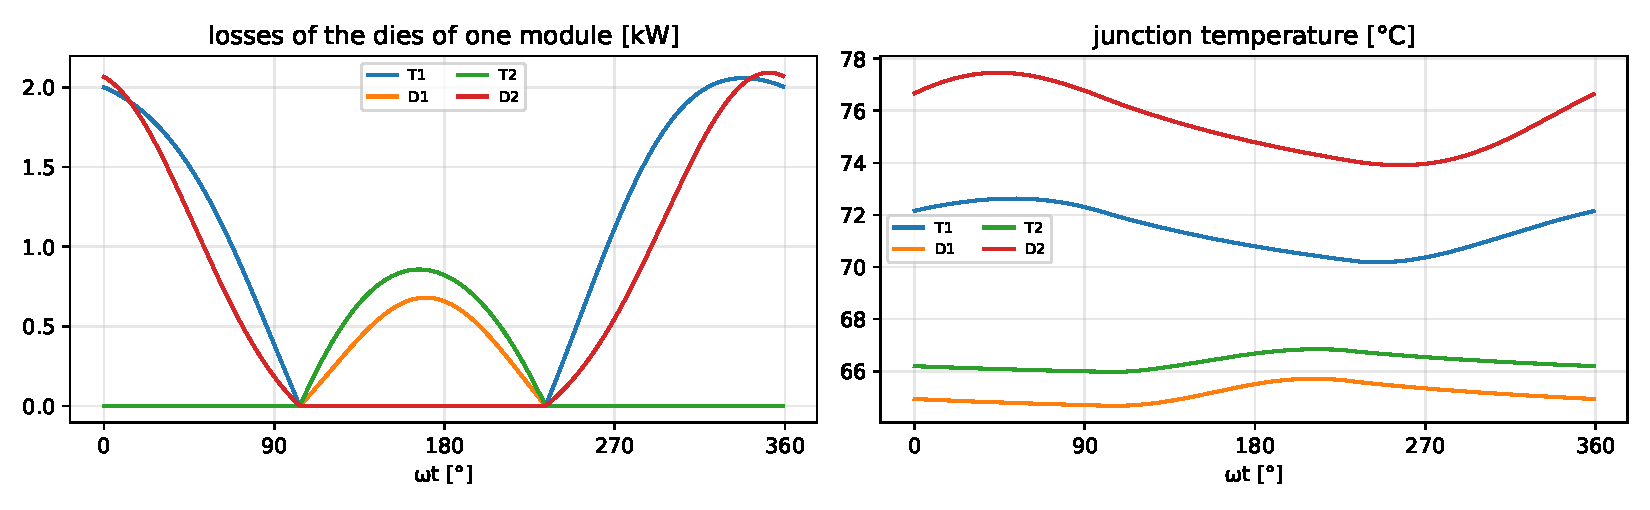
\includegraphics[width=\linewidth]{thermal/fig/junction_waveforms.pdf}
  \caption{Losses and junction temperatures of the dies over one period, example as in Table~\ref{tab:thermal-modules}}
  \label{fig:junction}
\end{figure}

Table~\ref{tab:thermal-flow} gives the highest junction temperature against the water flow per cold plate and the
inlet temperature. The inlet temperature adds one to one; halving the flow from 10\,l/min to 5\,l/min raises the
highest junction temperature by 8.3\,K.

\begin{table}[!ht]
  \centering
  \small
  \begin{tabular}{@{}r r r r@{}}
    \toprule
    \multicolumn{1}{c}{\textbf{$Q_w$ [l/min]}} & \multicolumn{1}{c}{\textbf{$T_{w\_in} = 40\,^{\circ}$C}}
      & \multicolumn{1}{c}{\textbf{50\,$^{\circ}$C}} & \multicolumn{1}{c}{\textbf{60\,$^{\circ}$C}} \\
    \midrule
    \tablerows{thermal/fig/flow_table}
    \bottomrule
  \end{tabular}
  \caption{Highest junction temperature in $^{\circ}$C against water flow per cold plate and inlet temperature}
  \label{tab:thermal-flow}
\end{table}
\FloatBarrier

